\documentclass[12pt]{article}
\usepackage[letterpaper, landscape, margin=0.5in]{geometry}
\usepackage{amsmath, amsthm, graphicx, tikz, pdflscape} 

\tikzset{
  treenode/.style = {shape=rectangle, %rounded corners,
                     draw, align=center,
                     top color=white, bottom color=blue!20},
  dec/.style = {%shape=text, rounded corners,
                    draw, align=center,
                    top color=white, bottom color=blue!20},
  root/.style     = {treenode, font=\Large, bottom color=red!30},
  env/.style      = {dec, font=\ttfamily\normalsize},
  dummy/.style    = {circle,draw}
}


\setlength\parindent{0pt}

\usepackage{fancyhdr}
\pagestyle{fancy}
\fancyhf{}
\lhead{Darshan Patel}
\rhead{Data Mining}
\renewcommand{\footrulewidth}{0.4pt}
\cfoot{\thepage}

\begin{document}

$$ 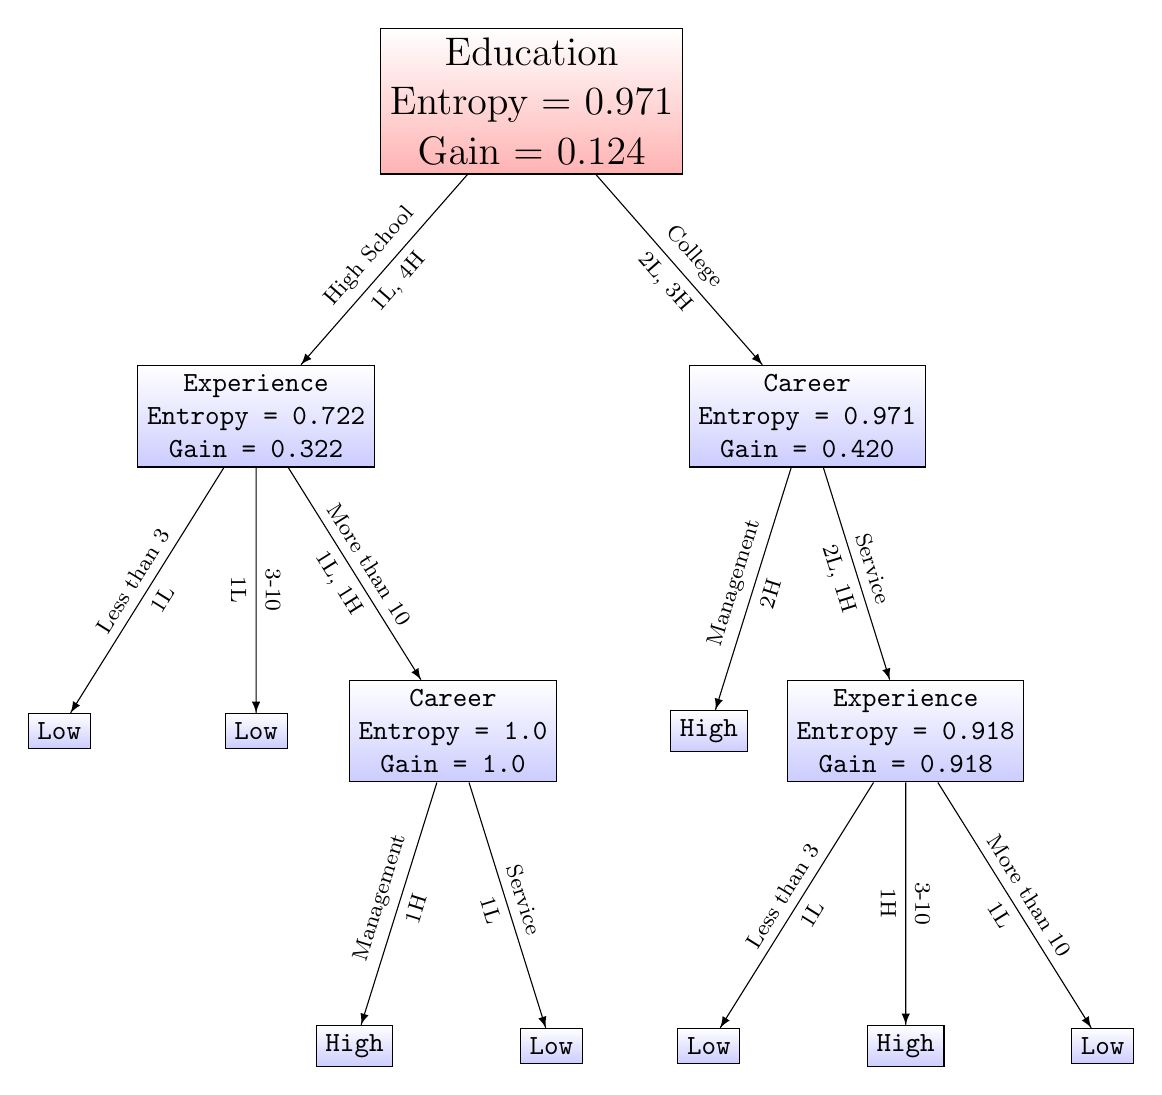
\begin{tikzpicture}
  [
  grow = down, 
  %sibling distance = 4cm,
 %level distance = 6cm,
  edge from parent/.style = {draw, -latex}, 
  every node/.style = {font = \footnotesize},
  sloped
  ]  
  
  \tikzstyle{level 1}=[sibling distance=70mm, level distance = 40mm] 
  \tikzstyle{level 2}=[sibling distance=30mm, level distance = 40mm]  
  \tikzstyle{level 2}=[sibling distance=25mm, level distance = 40mm]  


  
  \node[root] {Education \\ Entropy = 0.971 \\ Gain = 0.124} 
  	child{node [env] {Experience \\ Entropy = 0.722 \\ Gain = 0.322}
		child{node [env] {Low}
			edge from parent node [above] {Less than 3}
			edge from parent node [below] {1L} }
		child{node [env] {Low}
			edge from parent node [above] {3-10}
			edge from parent node [below] {1L} }
		child{node [env] {Career \\ Entropy = 1.0 \\ Gain = 1.0}
			child{node [env] {High}
				edge from parent node [below] {1H}
				edge from parent node [above] {Management} }
			child{node [env] {Low}
				edge from parent node [below] {1L}
				edge from parent node [above] {Service} }
			edge from parent node [above] {More than 10}
			edge from parent node [below] {1L, 1H} }
		edge from parent node [above] {High School} 
		edge from parent node [below] {1L, 4H} }
	child{node [env] {Career \\ Entropy = 0.971 \\ Gain = 0.420}
		child{node [env] {High}
			edge from parent node [below] {2H}
			edge from parent node [above] {Management} }
		child {node [env] {Experience \\ Entropy = 0.918 \\ Gain = 0.918}
			child{node [env] {Low}
				edge from parent node [above] {Less than 3}
				edge from parent node [below] {1L} }
			child{node [env] {High}
				edge from parent node [above] {3-10}
				edge from parent node [below] {1H} }
			child{node [env] {Low}	
				edge from parent node [above] {More than 10} 
				edge from parent node [below] {1L} }
			edge from parent node [below] {2L, 1H}
			edge from parent node [above] {Service} }
		edge from parent node [above] {College} 
		edge from parent node [below] {2L, 3H} };
		
\end{tikzpicture} $$ 

\newpage

$$ 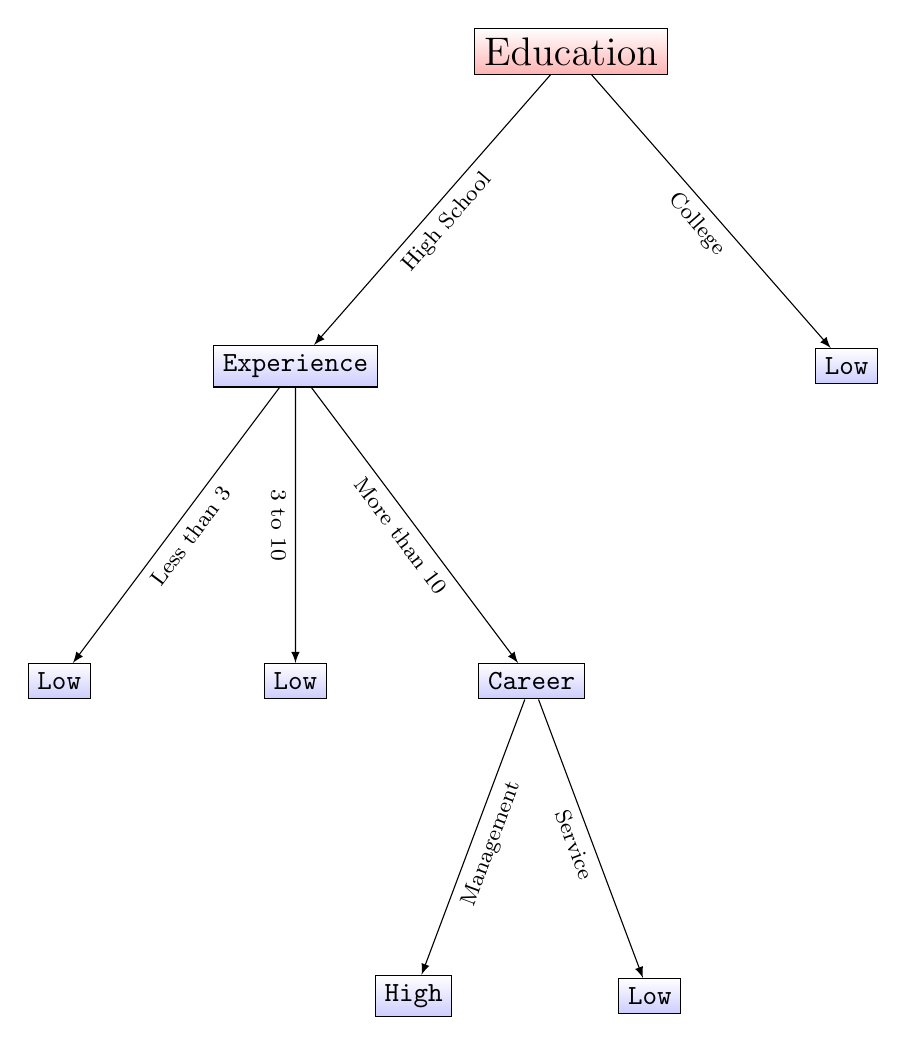
\begin{tikzpicture}
  [
  grow = down, 
  %sibling distance = 4cm,
 %level distance = 6cm,
  edge from parent/.style = {draw, -latex}, 
  every node/.style = {font = \footnotesize},
  sloped
  ]  
  
  \tikzstyle{level 1}=[sibling distance=70mm, level distance = 40mm] 
  \tikzstyle{level 2}=[sibling distance=30mm, level distance = 40mm]  
  
  \node[root] {Education}
  	child{node [env] {Experience}
		child{node [env] {Low} 
			edge from parent node [below] {Less than 3} } 
		child{node [env] {Low}
			edge from parent node [below] {3 to 10} } 
		child{node [env] {Career} 
			child{node [env] {High}
				edge from parent node [below] {Management} }
			child{node [env] {Low} 
				edge from parent node [below] {Service} }
			edge from parent node [below] {More than 10} } 
		edge from parent node [below] {High School} }
	child{node [env] {Low}
		edge from parent node [below] {College} } ;		
\end{tikzpicture} $$ 

\end{document} 				
				
				